\documentclass[11pt,a4paper]{article}
\usepackage[utf8]{inputenc}
\usepackage{amsmath}
\usepackage{amsfonts}
\usepackage{amssymb}
\usepackage{float}
\usepackage{graphicx}
\usepackage[ngerman]{babel}
\usepackage[a4paper, portrait, margin=1.2in]{geometry}
\author{Aaron Winziers (1176638), Thomas Schimper (1184921), Christopher Schmitt (1192978), Amir Durguti (1172920), Rudolf Barth}
\title{Großes Studienprojekt}
\begin{document}
\maketitle
\begin{abstract}
  Da IPv4 aufgrund von immer weiter steigenden Nutzerzahlen
  und internetfähigen Geräte bald nicht mehr als
  Standardadressraum verwendet werden kann und IPv6 eine
  mögliche Lösung dieses Problems ist, haben wir uns innerhalb
  unseres großen Studienprojektes mit dem Aufsetzen und
  Verwalten eines IPv4 bzw. IPv6 Netzwerkes
  auseinandergesetzt.
\end{abstract}
\section{Fragestellung}
Um sich mit dem Zusammenspiel von Geräten innerhalb eines
Netzwerkes vertraut zu machen, war gefordert das folgende
Diagramm als Netzwerk umzusetzen:
\begin{figure}[ht]
  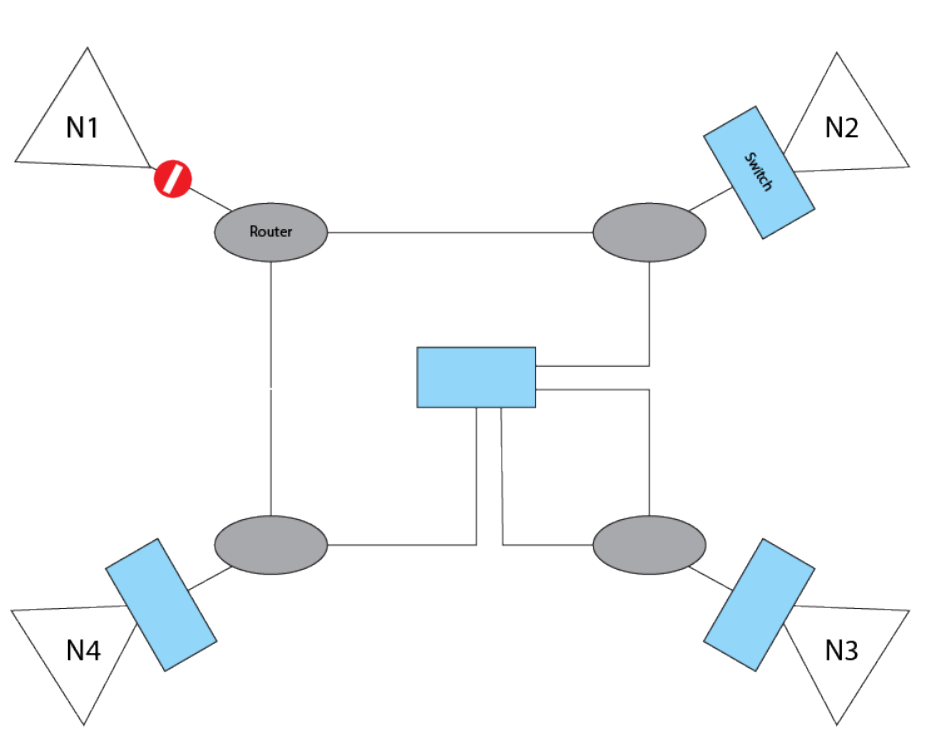
\includegraphics[width=\linewidth]{./network_topography.png}
  \centering
  \caption{Aufbau des Netzwerks}
\end{figure}
\par
Die mit N1 bis N4 beschriftete Dreiecke bezeichnen die von uns
erstellten Subnetze, die durch die Router (graue Ovale, R1 bis R4)
verwaltet werden, und die blauen Vierecke repräsentieren jeweils einen
Switch. Das \glqq Einfahrt Verboten\grqq~ Schild symbolisiert
zusätzlich eine von uns konfigurierte Firewall.
\par
Jeder Router verwaltet die Vergabe der IPs innerhalb der eigenen
Subnetze über einen eigenen DHCP-Server. Alle Router erkennen sich und
kommunizieren untereinander über statische Routen, wobei die
Kommunikation zwischen R2 und R4 zwei Hops (über R1) benötigt.
Außerdem werden die Verbindungen zwischen R2 und R3, und R3 und R4
über einem Switch und durch zwei unabhängige VLANs realisiert, die
über den Switch in der Mitte konfiguriert werden.
\par
Hinter R1 ist eine Verbindung zum Internet, die durch die Firewall
geschützt wird, welche durch den Gebrauch von \texttt{iptables}
realisiert wurde. Die Firewall ist so konfiguriert, dass sie den
ausgehenden Verkehr nicht einschränkt, jedoch eingehende Pakete
weiterleitet, wenn sie im Zusammenhang mit ausgehenden Paketen stehen.
\par
Der innere Switch sollte zusätzlich so konfiguriert sein das er die
Verbindungen zu den Routern über die verbliebene Ports spiegelt.

\section{Herangehensweise}
Nach ersten Recherchen bezüglich der Router und deren Funktionsweise
fiel uns auf, dass diese mit einer veralteten Firmwareversion
ausgestattet waren. Deshalb war der erste Arbeitsschritt das
Aktualisieren der Firmware. Die jetzt aktualisierte Firmware verfügte
über eine GUI, mit deren Hilfe jegliche Einstellungen bezüglich der
IPv4-Einstellungen konfiguriert werden konnten.
\par
Bevor die Aufgabe bearbeitet wurde war eine Einarbeitung in die
Funktionen und Eigenschaften des Systems erforderlich, um eine
vollständige Umsetzung der Fragestellung zu realisieren. Dazu wurde
ein simples Netzwerk mit Hilfe der Konsole konfiguriert. In diesem
Netzwerk wurden alle für die Aufgabenstellung wichtige
Komponenten (z.B. DHCP, Firewall, Static Routes, usw.) eingebunden, um
ein tieferes Verständnis dieser zu gewinnen.
\par
Nach ersten Konfigurationen wurde mit Hilfe der GUI geprüft, ob alle
Einstellungen erfolgreich übernommen wurden. Weil das Konfigurieren
der Router über die GUI deutlich einfacher und übersichtlicher ist,
wurde zur Umsetzung der Aufgabenstellung eine Kombination aus Konsole
und GUI verwendet.
\par
Bei der Bearbeitung der Aufgabe musste zu aller erst das Netzwerk auf
physischer Ebene, wie auf Abbildung 1 zu sehen, zusammengesetzt
werden. Dabei war eine übersichtliche Verkabelung wichtig, um die
Subnetze auch unproblematisch unterscheiden und visualisieren zu
können. Des Weiteren wurden die Router etikettiert um weitere
Übersicht und Organisation zu erschaffen.
\par
Wichtig war die Dokumentation des Verlaufs der Umsetzung, als auch
eine Möglichkeit ältere Konfigurationen zu sichern und wieder
herzustellen. Hierzu wurde Git auf dem berühmten Hostingplattform
Github verwendet, dies erlaubte eine bessere Organisation des Projekts
und effektivere Zusammenarbeit.


\section{Konfiguration}
R0 dient als Schnittstelle zum Internet, deshalb ist er der
einzige Router, welcher kein eigenes Subnetz aufspannt. Im Gegensatz zu
den anderen Routern konnte an eth1 und eth2 (die Verbindung zu R1 und
R2) keine festen IP-Adressen vergeben werden. Stattdessen läuft ein
DHCP-Server, der dem jeweiligen Anschluss eine passende IP-Adresse
vergibt. Das ist notwendig, da sonst kein Zugriff auf das Webinterface
des Routers mehr möglich wäre. Die drei anderen Router sind über eine
IP-Adresse aus dem Adressraum ihres jeweiligen Subnetzes erreichbar
(z.B. Router 3: 192.168.3.1) \par
	
R1-R3 haben alle eine recht ähnliche Konfiguration: alle bieten
auf eth0 ein eigenes Subnetz. Über eth1 und eth2 sind sie mit den
anderen Routern verbunden. Die Router sowie die Geräte in den
Subnetzen können sich über statische Routen erreichen.
\par
	
Die Firewall wurde entsprechend der Vorgabe in der Aufgabenstellung
konfiguriert. Die Konfiguration erfolgte hauptsächlich über die in der
Router-Software verfügbare Shell. Diese ist wesentlich mächtiger als
das integrierte Webinterface, insbesondere bei seltener verwendeten
Features des Routers.
\par
	
Das VLAN wurde durch die Konfiguration des entsprechenden Switches
realisiert. Dies lässt sich mit der Konfigurationssoftware
bewerkstelligen, die allerdings nur für Windows vorliegt (alternativ
geschieht die Konfiguration über ein Web-Interface). Unsere Lösung sah
zuerst vor, die Ports 1-4 und 5-8 als zwei VLANs zu trennen. Da wir
jedoch noch einen Port für das Monitoring benötigten, mussten wir das
zweite VLAN um einen Port verkleinern. Somit kann nun der gesamte
Traffic des Switches an Port 8 abgegriffen werden. \par


\section{Netzwerkanalyse}
Um die realisierte Topologie auf Korrektheit und Funktionalität zu
überprüfen, wurde nach der Konfiguration des gesamten Netzwerkes,
sowohl die Erreichbarkeit unter den einzelnen Geräten, als auch die
Verbindungsrouten selbst mit Hilfe verschiedener Methoden getestet.
\par
Um die Erreichbarkeit zu prüfen, haben wir versucht von einem Gerät
aus ein weiteres Gerät, welches in einem anderen Subnetz registriert
hatte, mittels des Unix-Tools \texttt{ping} zu erreichen. Um zu
verhindern, dass ein falsches Gerät als Ziel angegeben wurde, haben
wir uns zunächst die einzelnen IP-Adressen der jeweiligen Rechner mit
dem Konsolen-Befehl \texttt{ifconfig} beschafft und diese mit den
DHCP-Leases im entsprechenden Router überprüft. Die Tests verliefen
alle erfolgreich, was uns dazu führte, das Netzwerk weitergehend zu
untersuchen.
\begin{figure}[ht]
\begin{tabular}{|c|c|c|c|}
\hline 
Test & Ausgangsrechner & Zielrechner & Ergebnis \\ 
\hline 
Ping & hinter R2 & hinter R1 & erfolgreich \\ 
\hline 
Ping & hinter R2 & hinter R3 & erfolgreich \\ 
\hline 
SSH & hinter R2 & hinter R1 & erfolgreich \\ 
\hline 
SFTP & hinter R2 & hinter R1 & erfolgreich \\ 
\hline 
\end{tabular} 
  \centering
  \caption{Durchgeführte Tests}
\end{figure}
\par 
Bevor wir jedoch TCP oder UDP basierende Pakete über die internen
Leitungen versendet haben, richteten wird zunächst einen uns zur
Verfügung gestellten Rasberry Pi ein, sodass dieser einen
OpenSSH-Server bereitstellte. Dieser wurde dazu benutzt um SSH und
SFTP-Anfragen zu realisieren. Um weitergehende Informationen zu
erhalten, wurde ein dritter Rechner (A1) am Mirror-Port des Switches
mit den VLANs eingebunden, dieser mit dem Tool \texttt{Wireshark} die
pVerbindungen und Übertragungen analysierte.
\begin{figure}[H]
  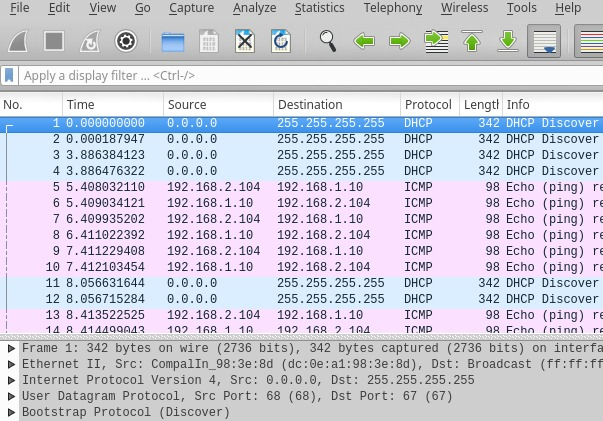
\includegraphics[width=\linewidth]{./wireshark1.jpeg}
  \centering
  \caption{Analyse von Pings mittels \texttt{Wireshark}}
\end{figure}
\begin{figure}[H]
  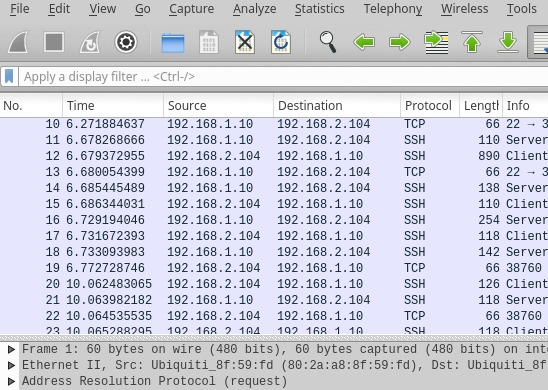
\includegraphics[width=\linewidth]{./wireshark2.jpeg}
  \centering
  \caption{Analyse von SSH-Verbindungen mittels \texttt{Wireshark}}
\end{figure}
\par
Die Verbindung über Ping (ICMP), \texttt{SSH} oder auch \texttt{SFTP}
von R1 nach R3 verursachte bei A1 keinen angezeigten Datenverkehr, was
zu erwarten war, da R0, R1 und R3 über Static Routes direkt
kommunizieren können und keine Daten über den Switch versendet werden.
Alle anderen Verbindungen, welche über oder mit R2 hergestellt wurden
zeigten bei den jeweiligen Tests die zu erwartenden Protokolle und
Daten an. Bei den Versuchen mit \texttt{ping} kam das ICMP-Protokoll
zum tragen. Bei den SSH und SFTP Verbindungen wurde \texttt{TCP} und
\texttt{SSH} verwendet, jedoch war die Gewichtung der einzelnen Pakete
unterschiedlich. So war die Paketverteilung von SSH zu TCP beim
SSH-Test ungefähr 2 zu 1, wohingegen beim SFTP-Test der Anteil an SSH
Paketen wesentlich höher war.


\section{Evaluation \& Fazit}
Der erste Teil des großen Praktikums erwies sich als günstiger
Einstieg, um effizient den Umgang mit dem IPv4-Protokoll und
allgemeinen Netzwerkarchitekturen zu erlernen. Wenn man zu beginnt
vielleicht gedacht haben sollte, dass das Einrichten eines Netzwerkes
bloß Plug-and-Play sei, mag dies vielleicht für einfache Netzwerke mit
nur einem Router gelten. Betreibt man jedoch wie bei uns verlangt
mehrere Router mit verschiedenen Subnetzen, so zeigt sich die
Komplexität der Netzwerkkonfiguration. Um die Aufgabenstellung wie
gefordert absolvieren zu können mussten wir zunächst lernen, wie wir
die Router miteinander kommunizieren lassen konnten. Wir
konfigurierten zunächst einen Router so, dass dieser über einen
DHCP-Server automatisch IP-Adressen an Clients vergeben konnte. Als
sich unsere Geräte eine IP-Adresse automatisch vom Router beziehen
konnten, gingen wir dazu über zwei Router miteinander zu verbinden.
Damit Geräte in den zwei verschiedenen Subnetzen der Router
untereinander kommunizieren konnten und sich gegenseitig finden,
bedarf es dem Gebrauch von statischen Routen, damit die Router
wussten, wohin sie die Anfrage weiterleiten mussten.
\par
Mit dem neuerlangten Wissen begannen wir jetzt unser Projekt mit dem
Verbinden des Routers 0, der nicht nur als Gateway ins Internet
fungieren sollte, sondern auch eine Brücke zwischen Router 1 und 3
bildete. Wichtig dabei war es zu erkennen, dass der Router 0 nach
Abschluss der Konfiguration nicht mehr auf direktem Weg über den
Ethernet-Port \texttt{eth0} erreicht werden konnte, da dieser dafür
benutzt wurde, um eine Verbindung zum Internet herzustellen.  Nach
ausreichender Konfiguration überbrückte der Router Anfragen auf
\texttt{eth1} and \texttt{eth2} und andersherum. Über die gemeinsam
genutzte Schnittstelle \texttt{eth0} konnte eine Verbindung mit dem
Internet hergestellt werden.
\par
Als letzten Teil der Aufgabe kam der 8-Port-Switch von NetGEAR zum
Einsatz. Dieser sollte die Ports eins und zwei zu einem VLAN
hinzufügen und die Ports drei und vier in ein zweites. In dem ersten
VLAN sollten die Router 2 und 3 kommunizieren und auf dem zweiten
Router 1 und 2. Zusätzlich wurden alle Ports auf denen Traffic
erfolgen könnte auf den Port 8 gespiegelt. Über diesen Port konnten
wir mittels Wireshark Traffic analysieren und speichern, was wir auch
im Teil der Netzwerkanalyse getan haben.
\par
Der ersten Teil des Projekts wies uns in die Grundlagen des
IPv4-Protokoll ein und bereitete uns darauf vor, das vorgegebene
Netzwerk auf das IPv6-Protokoll zu portieren. Wir eigneten uns nicht
nur neue Fähigkeiten im Umgang mit Netzarchitekturen, sondern lernten
auch den Umgang mit embedded Linuxsystemen und die Verwendung von Git.


\end{document}
